%TODO: add cliffhanger with preview for next time

%variability
%code-generation
%testing

%modularity? + dependences

% Make nice A4 pages for print:
%\usepackage{pgfpages}
%\pgfpagesuselayout{resize to}[a4paper,border shrink=5mm,landscape]

\beamertemplatenavigationsymbolsempty

\setbeamertemplate{bibliography item}[text]

\usepackage[type={CC},modifier={by-sa},version={4.0}]{doclicense}

\usepackage[utf8]{inputenc}
\usepackage{hyperref}
\usepackage{breakurl}
\usepackage{graphicx}
\usepackage{pgfplots}
\usepackage{pgf}
\usepackage{tikz}
\usetikzlibrary{positioning}
\usetikzlibrary{arrows}
\usetikzlibrary{decorations.markings}
\usetikzlibrary{calc}
\usetikzlibrary{matrix}
\usetikzlibrary{shapes}
\usetikzlibrary{decorations.pathmorphing}
\usetikzlibrary{fit}
\usetikzlibrary{backgrounds}
\usetikzlibrary{plotmarks}
\usepackage{stmaryrd}
\usepackage{listings}
\usepackage{pdflscape}
\usepackage{perpage}
\usepackage{appendixnumberbeamer}

%\usepackage[thmmarks,amsmath,amsthm]{ntheorem} % already included in beamer
\usepackage{thm-restate}

\usepackage[sort&compress,numbers]{natbib}  % to be have \citet, \citeauthor, \citeyear

\MakePerPage{footnote}

\tikzstyle{o}=[r,ppBlue]
\tikzstyle{r}=[thick,rectangle,align=center]
\tikzstyle{t}=[r,ppTrans] %,font=\bfseries]
\tikzstyle{dd}=[densely dashed]
\tikzstyle{n}=[r,ppBlue]
\tikzstyle{p}=[r,ppRed]
\tikzstyle{ppRed}  =[draw=red,  fill=  red!20]
\tikzstyle{ppBlue} =[draw=blue, fill= blue!20]
\tikzstyle{ppGreen}=[draw=green,fill=green!20]
\tikzstyle{ppTrans}=[draw=none, fill=none]

\usetheme{Warsaw}

\useoutertheme[subsection=true]{smoothbars}
%\useoutertheme[subsection=false]{miniframes}

\definecolor{bblue}{HTML}{D7DF01}	% yellow-ish actually, for better black/white printing
\definecolor{rred}{HTML}{C0504D}
\definecolor{ggreen}{HTML}{9BBB59}
\definecolor{ppurple}{HTML}{9F4C7C}
\definecolor{lightgray}{rgb}{0.3,0.3,0.3}
\definecolor{lightergray}{rgb}{0.9,0.9,0.9}
\definecolor{UniBlue}{RGB}{83,121,170}

\DeclareTextFontCommand\textintro{\normalfont\bfseries\itshape} % nice!
\newcommand{\intro}[2][]
{%
	\textintro{#2}%
}
\newcommand{\empha}[2][]
{%
	\emph{#2}%
}

%\theoremstyle{plain}
\newcounter{reqcounter}
\newtheorem{requirement}[reqcounter]{Requirement}

%setbeamercolor{structure}{fg=violet}

\makeatletter
\def\th@task{%
    \normalfont % body font
    \setbeamercolor{block title example}{bg=orange,fg=white}
    \setbeamercolor{block body example}{bg=orange!20,fg=black}
    \def\inserttheoremblockenv{exampleblock}
  }
\makeatother

\theoremstyle{task}
\newtheorem{task}{Task}

\newenvironment{assignment}%
{%\setbeamercolor{background canvas}{bg=violet}%
%\setbeamercolor{structure}{fg=cyan!90!black}%
 \setbeamercolor{frametitle}{bg=orange,fg=white}
\begin{frame}}%
{\end{frame}}%

\AtBeginSection[]{
  \begin{frame}
  \vfill
  \centering
  \begin{beamercolorbox}[sep=8pt,center,shadow=true,rounded=true]{title}
    \usebeamerfont{title}\insertsectionhead\par%
  \end{beamercolorbox}
  \tableofcontents
  \vfill
  \end{frame}
}




\pgfplotsset{compat=1.14}
\author{Markus Raab}


\date{23.3.2018}

\begin{document}

\renewcommand{\enquote}[1]{\emph{``#1''}} % Cannot be done earlier

%%%%%%%%%%%%%%%%%%%%%%%%%%%%%%%
\begin{frame}
	\titlepage
	\doclicenseThis
\end{frame}

\begin{frame}
	\frametitle{Organization}
	Next dates:
	\begin{description}
		\item[23.3.2018:] \textbf{teams found together, dates of talks}
		\item[13.4.2018:] homework submitted, topics of team exercise
		\item[27.4.2018:] lecture
		\item[4.5.2018:] lecture
		\item[18.5.2018:] guest lecture
		\item[25.5.2018:] team exercise submitted
		\item[1.6.2018:] lecture
		\item[8.6.2018:] lecture
		\item[15.6.2018:] \textbf{last corrections of team exercise}
		\item[22.6.2018:] \textbf{test}
	\end{description}
\end{frame}

\begin{frame}[fragile]
	\frametitle{Recapitulation}

	\begin{itemize}[<+-| alert@+>]
	\item alarming trend in number and complexity of configuration settings
	\item sharing, visibility and default value calculation often helps
	\item needs abstraction: configuration specification
	\item but also more courageous decisions and periodical reevaluation
	\item different ways to reduce configuration space
	\end{itemize}
\end{frame}

\begin{frame}
	\frametitle{Recapitulation (Metalevels)}
	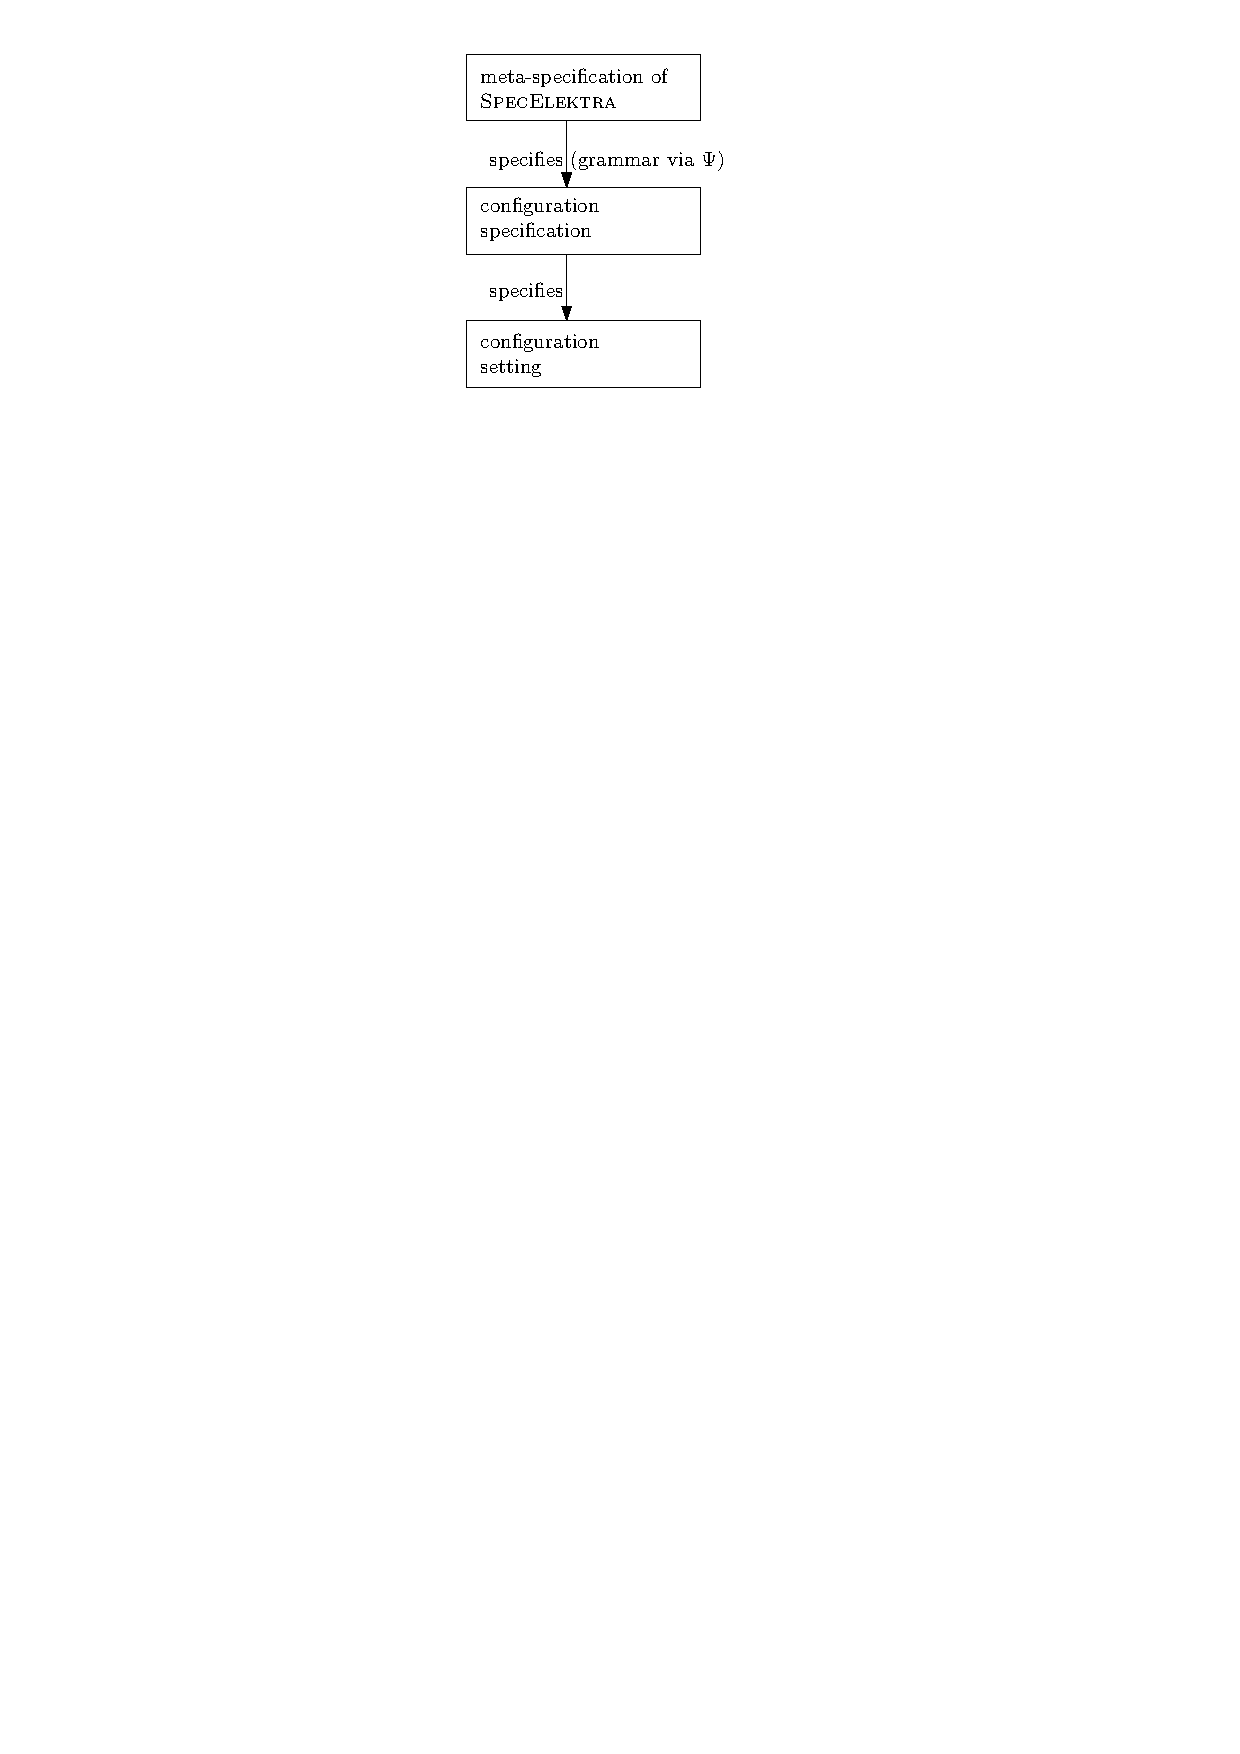
\includegraphics{metalevels}
\end{frame}

\begin{frame}
	\Large
	\ExecuteMetaData[../book/approach.tex]{definition-spec}
\end{frame}

\begin{frame}
	\frametitle{Recapitulation (Requirements of SpecElektra)}

	\begin{itemize}
	\item formal and informal
	\item should strive for completeness
	\item should be extensible
	\item should be external to application
	\item open for introspection (for tooling)
	\item should talk to users
	\item should allow generation of artefacts
	\end{itemize}
\end{frame}


\begin{frame}
	\frametitle{Popular Topics}
	\vspace{-0.5cm}
	\begin{multicols}{2}
	\begin{description}
	\item[4] validation
	\item[4] user interface
	\item[3] tools (benefits?)
	\item[3] testability
	\color{gray}
	\item[3] complexity reduction (when conf. needed?)
	\item[3] architectural decisions
	\color{black}
	\item[2] Puppet
	\color{red}
	\item[2] modularity
	\color{gray}
	\item[2] environment variables
	\color{black}
	\item[2] documentation
	\color{red}
	\item[2] configuration specification
	\color{gray}
	\item[2] command-line args\color{black}
	\item[2] code generation
	\item[1] variability
	\item[1] self-description
	\item[1] round-tripping
	\color{red}
	\item[1] introspection
	\item[1] dependences
	\item[1] auto-detection
	\color{black}
	\item[1] early
	\item[1] context-awareness
	\item[1] administrators
	\end{description}
	\end{multicols}
\end{frame}

\begin{frame}
	\frametitle{Goals for today}
	\begin{itemize}
	\item modularity on system level
	\begin{itemize}
	\item horizontal
	\item vertical
	\end{itemize}
	\item system-wide introspection
	\item avoiding dependences
	\item auto-detection
	\end{itemize}
\end{frame}




%%%%%%%%%%%%%%%%%%%%%%%%%%%%%%%%%%%%%%%%%% 
\section{Modularity}

\subsection{Definitions}

\begin{frame}
	\Large
	\ExecuteMetaData[../book/background.tex]{definition-configuration-access}
\end{frame}

\begin{frame}[fragile]
	\frametitle{Configuration Access APIs}

	\begin{task}
	Which configuration access APIs do you know? \\
	What are the differences between these APIs?
	\end{task}

	For example:
	\begin{itemize}[<+-| alert@+>]
	\item ^char * getenv (const char * key)^
	\item ^ConfigStatus xf86HandleConfigFile(Bool autoconfig)^
	\item ^long pathconf (const char *path, int^ ^name)^
	\item ^long sysconf (int name)^
	\item ^size_t confstr (int name, char *buf, size_t len)^
	\end{itemize}
\end{frame}

%TODO: disadvantages in hard-coding configuration
%TODO: disadvantages in having transformations
%TODO: disadvantages in missing introspection

\begin{frame}[fragile]
	\ExecuteMetaData[../book/background.tex]{definition-configuration-access-points}

	\begin{code}[language=Cpp,gobble=4,showspaces=no]
	int main()
	{
		getenv ("PATH");
	}
	\end{code}
\end{frame}

\begin{frame}[fragile]
	\ExecuteMetaData[../book/background.tex]{definition-configuration-library}

	Trends:
	\begin{itemize}[<+-| alert@+>]
	\item flexibility to configure configuration access (e.g., \url{https://commons.apache.org/proper/commons-configuration/})
	\item more type safety (e.g., \url{http://owner.aeonbits.org/}, code generation in next lecture)
	\item try to unify something (UCI, Augeas, Elektra)
	\end{itemize}
\end{frame}

\begin{frame}
	\Large
	\ExecuteMetaData[../book/backend.tex]{definition-modularity}
\end{frame}

\subsection{Vertical}

\begin{frame}[fragile]
	\frametitle{Vertical Modularity \cite{raab2016improving}}

	\intro[modularity!vertical]{Vertical modularity} is the degree of separation between different applications.
	If all applications use the same key database with a single backend or a single configuration file, applications would be coupled tightly.
	[...]

	If coupling between applications is low, for example every application uses a different configuration library or a different backend, we have a high degree of vertical modularity.
\end{frame}


\begin{frame}
	\frametitle{Retain Modularity \cite{raab2016improving}}

	\elektra{} provides two mechanisms to retain vertical modularity:

	\begin{itemize}
	\item \textbf{Mounting} configuration files facilitates different applications to use their own backend and their own configuration file.
	Furthermore, mounting enables integrating existing configuration files into the key database.
	Configuration specifications written in \elektra{Spec} allow different applications to share their configuration files with each other in a controlled way.

	\item Having frontends that implement existing \textbf{APIs} decouple applications from each other.
	These applications continue to use their specific configuration accesses, but \elektra{} redirects their configuration accesses to the shared key database.
	\end{itemize}
\end{frame}

\begin{frame}[fragile]
	Mountpoints can also be a part of the specification:

	\begin{code}[language=Cpp,gobble=4,showspaces=no]
	[ntp]
	  mountpoint:=ntp.conf
	[sw/libreoffice]
	  mountpoint:=libreoffice.conf
	\end{code}

	\begin{task}
	Which type of specification is this?
	\end{task}
\end{frame}

\begin{frame}
	\frametitle{Types of Specifications}
	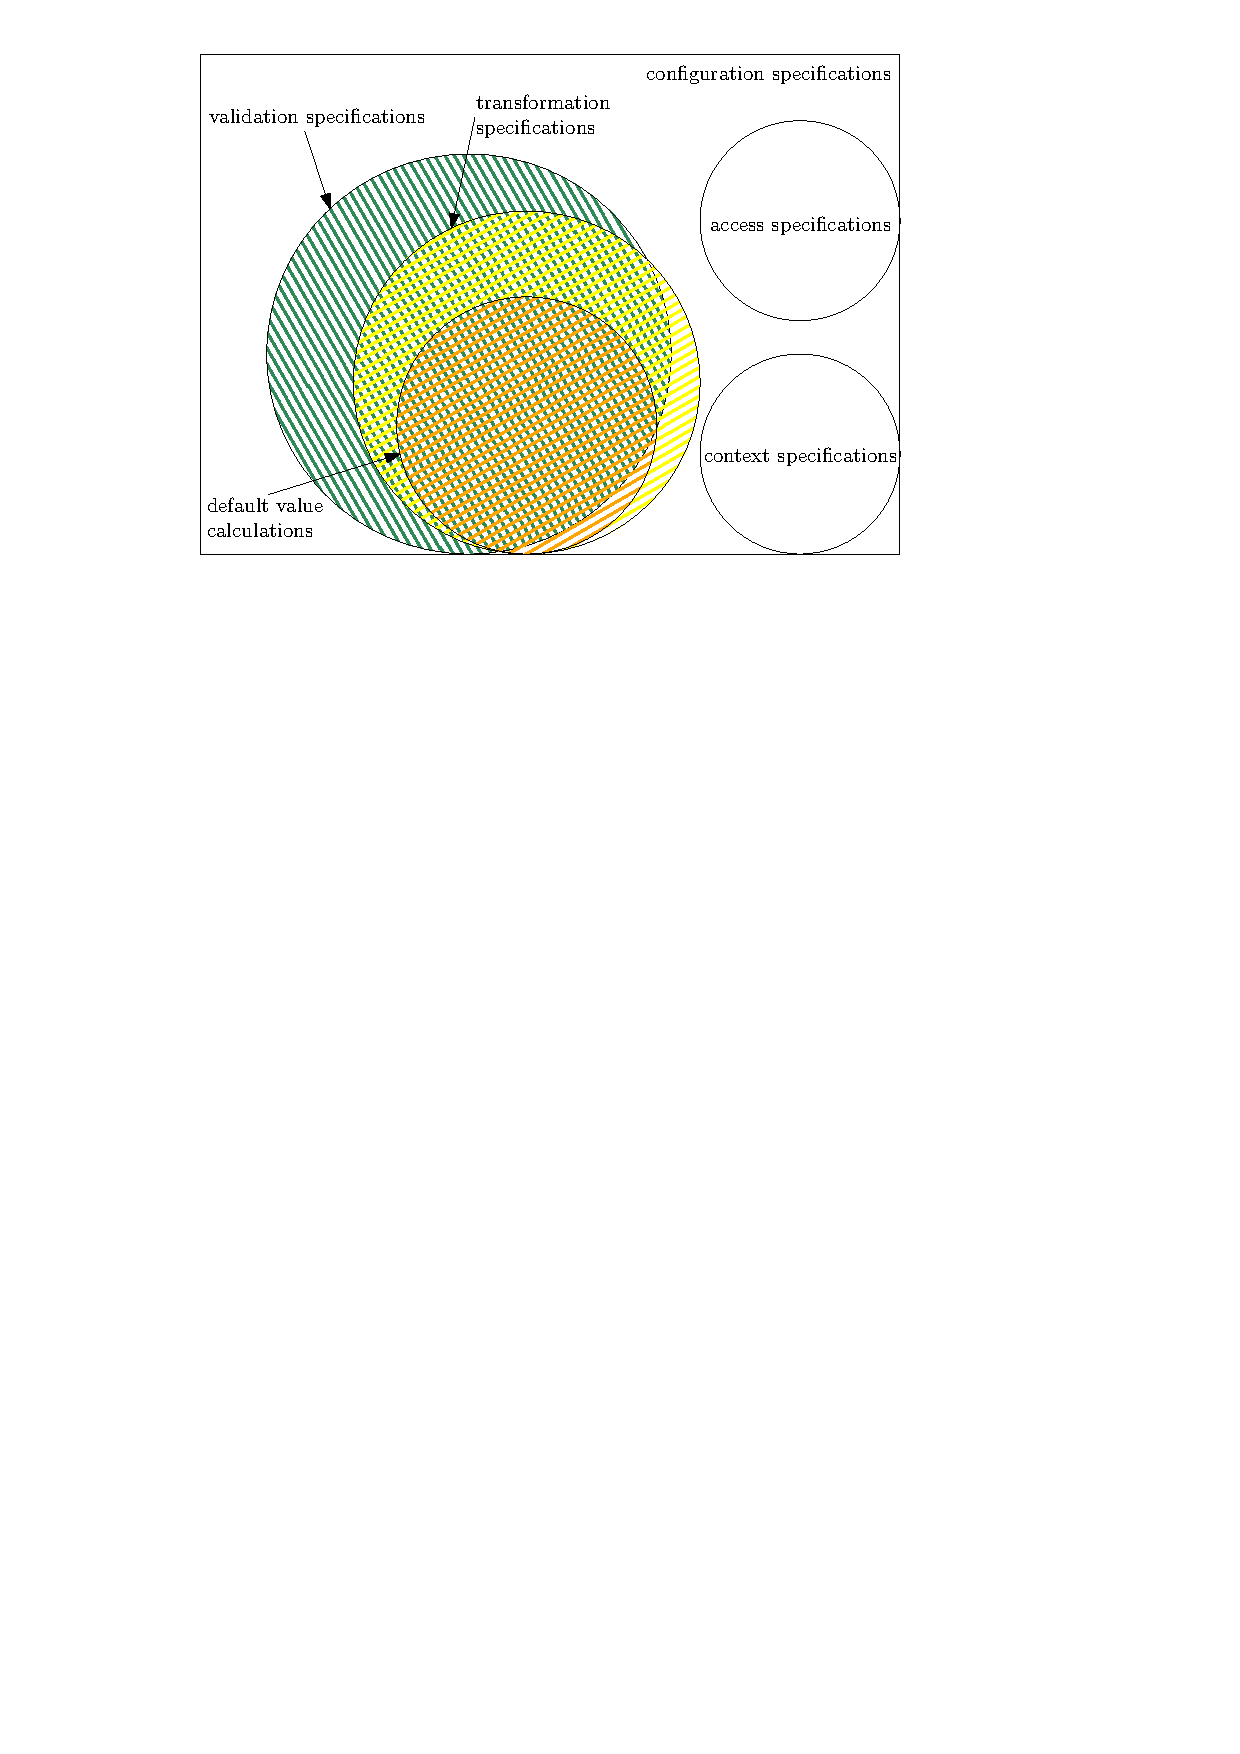
\includegraphics[scale=0.8]{specifications}
\end{frame}

\begin{frame}
	\frametitle{Vertical Modularity}
	\begin{columns}[c]
	\column{7cm}
	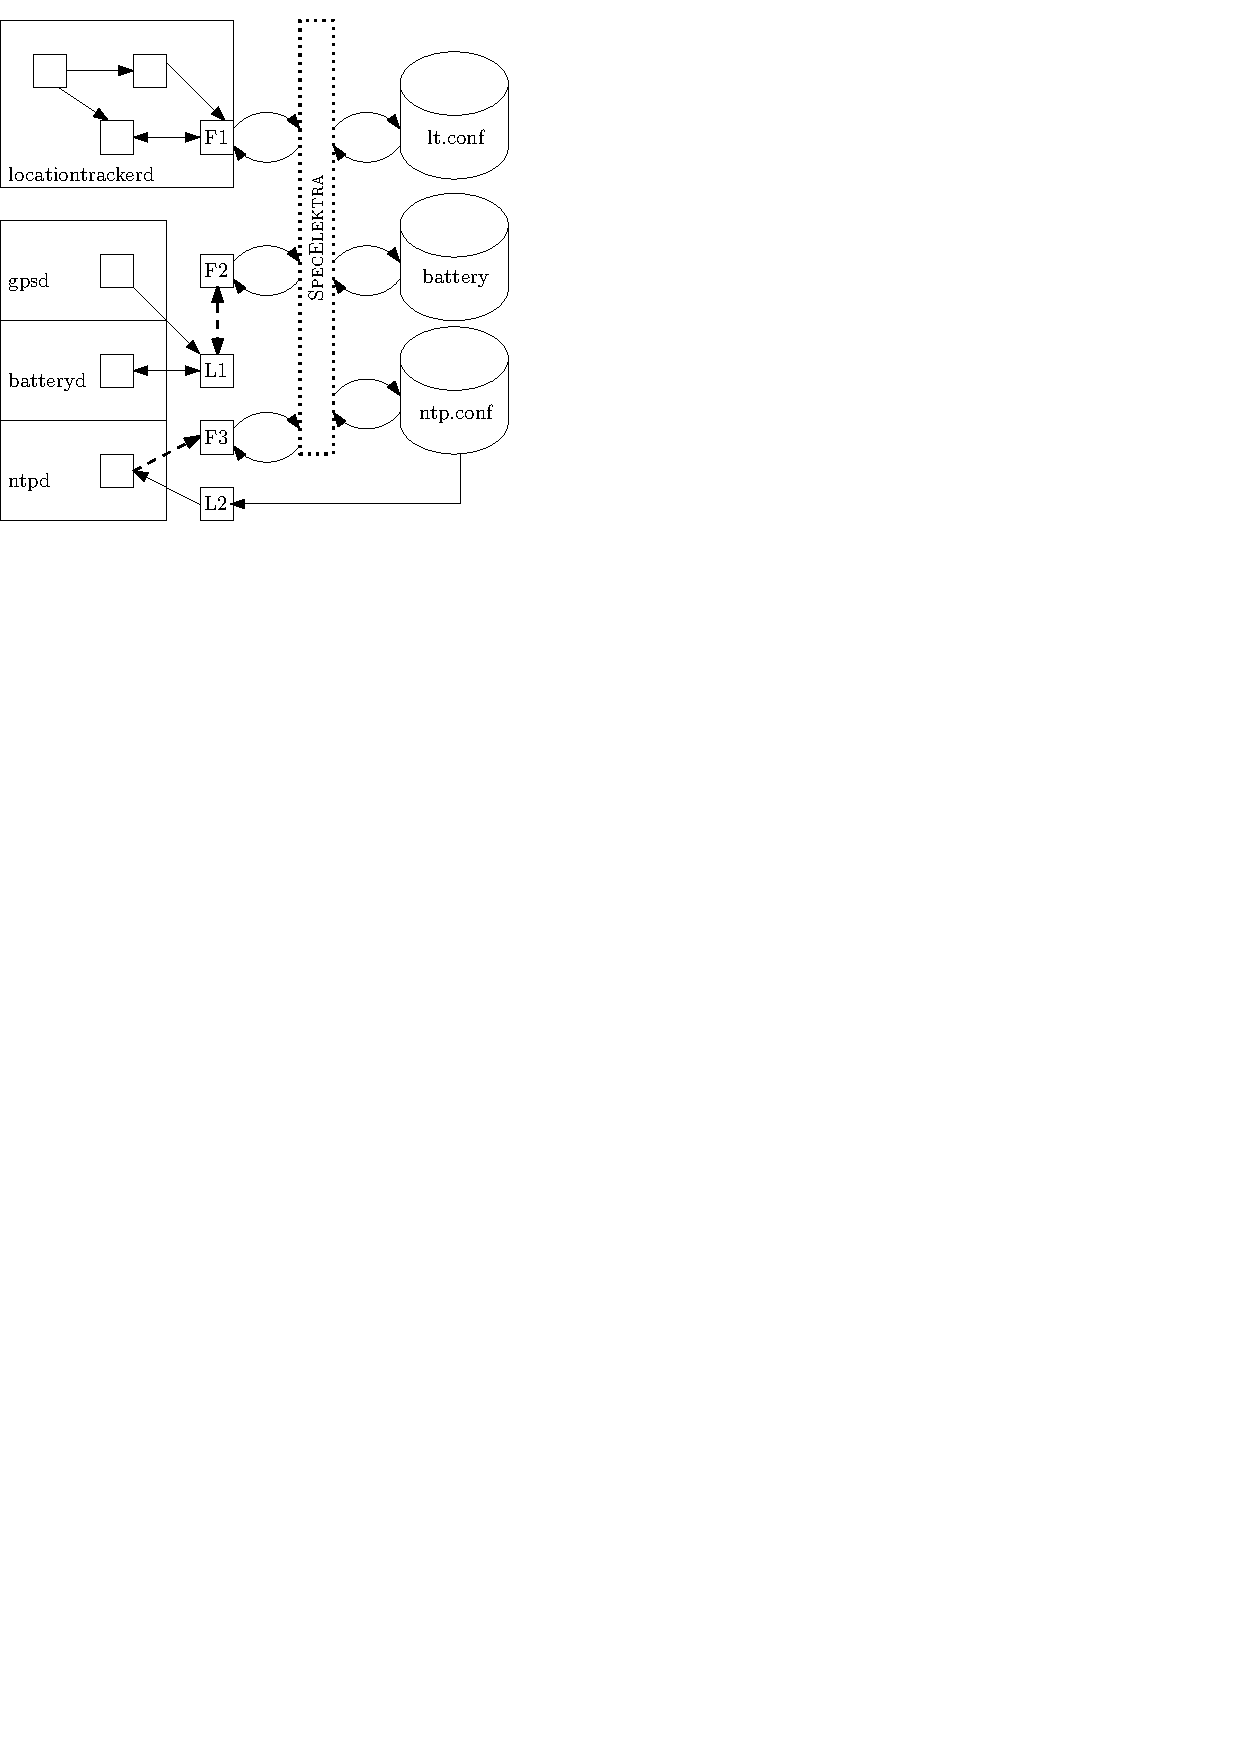
\includegraphics[scale=0.75]{verticalmodularity}
	\column{4cm}
	Needed to keep applications independently.

	Boxes are applications, cylinders are configuration files, F? are frontends or frontend adapters, L? are configuration libraries~\cite{raab2016improving}.
	\end{columns}
\end{frame}



\subsection{Horizontal}

\begin{frame}
	\intro[Modularity!horizontal]{Horizontal modularity} is ``the degree of separation in configuration access code''~\cite{raab2016improving}. 
	A higher degree of horizontal modularity allows us to better separate configuration access code and plug the code together as needed.
\end{frame}

\begin{frame}
	Three factors of \elektra{Spec} improve horizontal modularity:
	\begin{enumerate}
	\item
	Using \elektra{Spec}, applications are completely decoupled from configuration specifications.

	\item
	Specifications and their implementation are decoupled.

	\item
	Abstract dependences within the implementation of specifications.
	\end{enumerate}

	\begin{task}
	This is very vague.

	Can you describe a system that would (not) fulfil this?
	\end{task}
\end{frame}

\begin{frame}
	\frametitle{Horizontal Modularity}
	\begin{columns}[c]
	\column{7cm}
	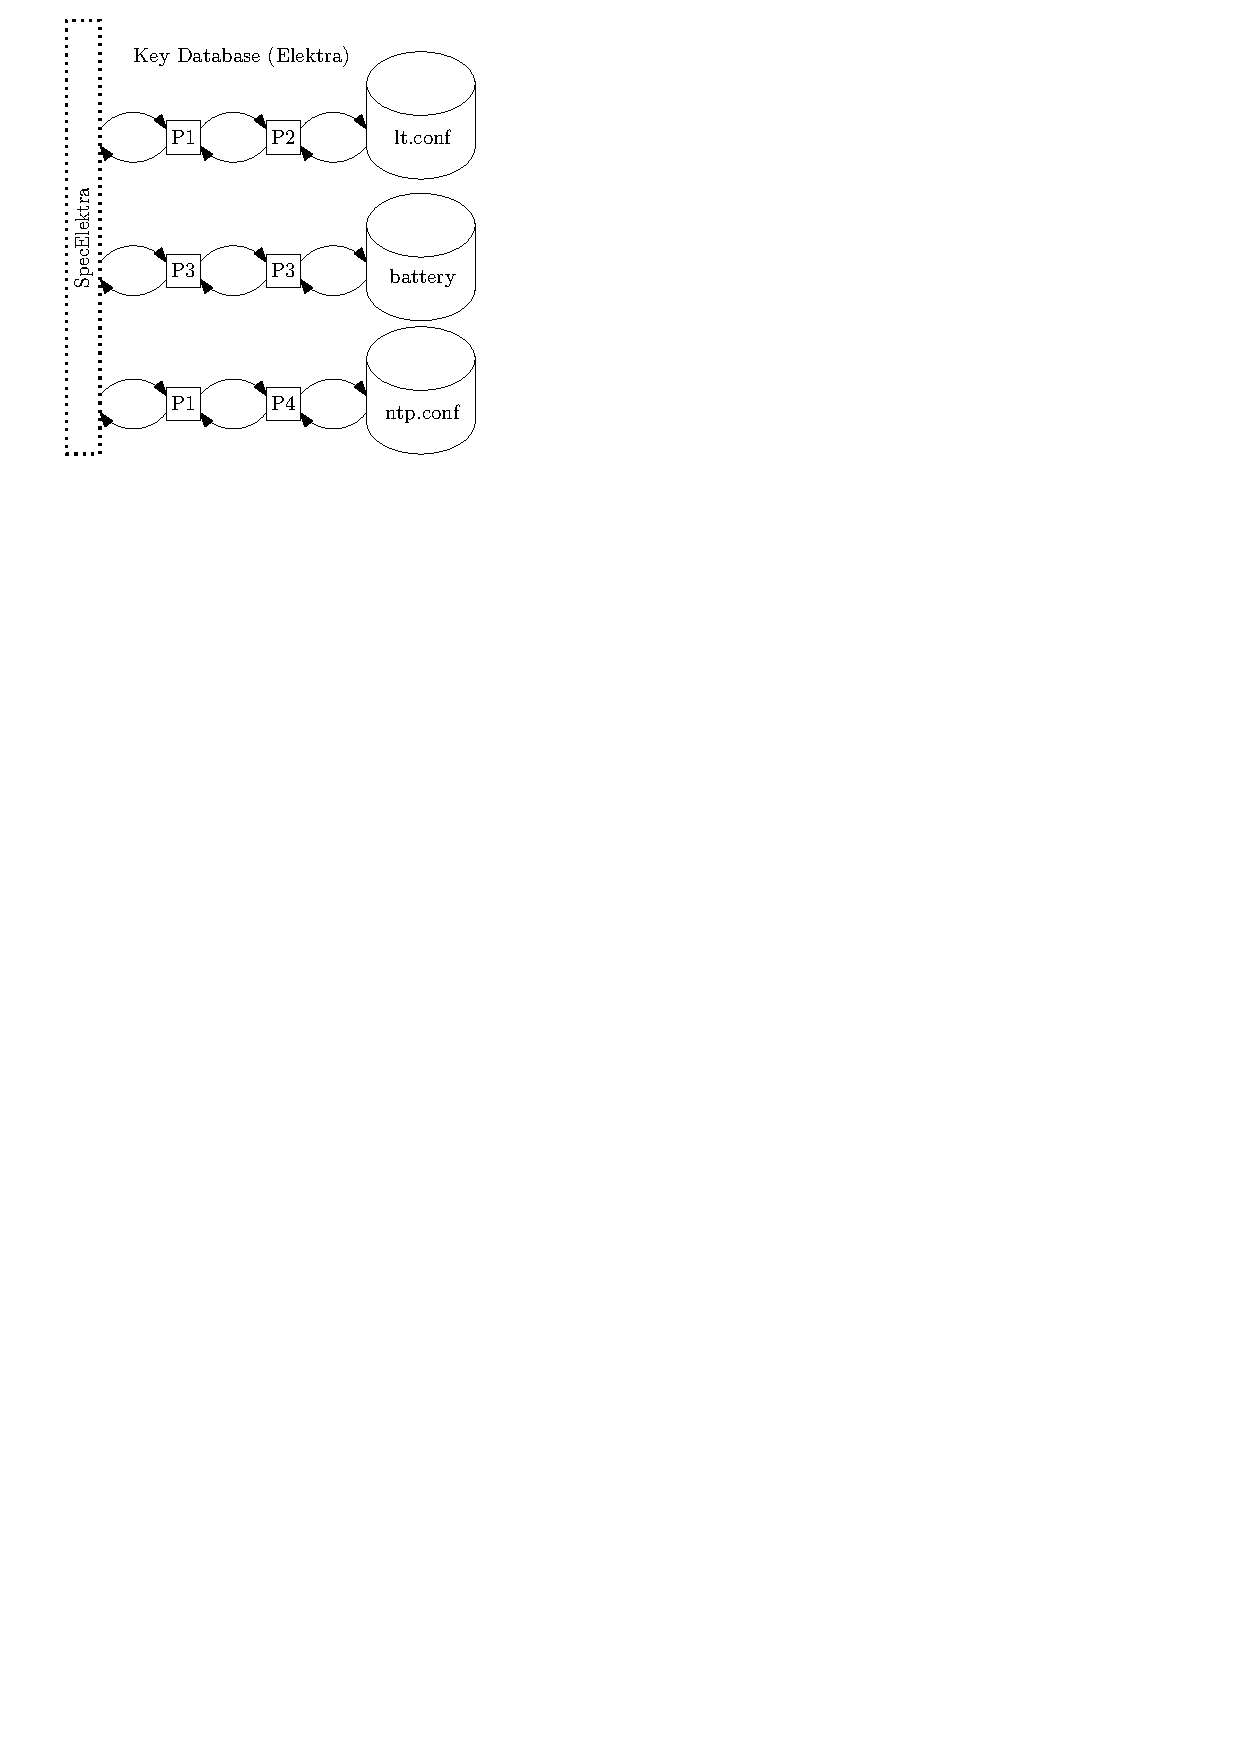
\includegraphics[scale=0.95]{horizontalmodularity}
	\column{4cm}
	Needed mainly for validation. \\[1cm]

	Cylinders are configuration files, P? are plugins~\cite{raab2016improving}
	\end{columns}
\end{frame}


%%%%%%%%%%%%%%%%%%%%%%%%%%%%%%%%%%%%%%%%%% 
\section{Plugins}

\subsection{Why?}

\begin{frame}
	\begin{finding}
	Most developers have concerns adding dependences for more validation~(\p{84}) but consider good defaults important (\p{80}).
	\end{finding}

	\begin{restatable}{requirement}{reqDependences}
	\label{req:dependences}
	Dependences exclusively needed to validate configuration settings must be avoided.
	\end{restatable}
\end{frame}

\begin{frame}
	\frametitle{Rationale}
	Why is it difficult to have good defaults?
	\begin{itemize}[<+->]
	\item modularity: diverse and conflicting requirements between applications %TODO: example
	\item system-level: specification must always be enforced
	\item Examples:
	\begin{itemize}[<+-| alert@+>]
	\item which desktop is the application started in?
	\item how many CPUs does the system have?
	\item get the correct proxy of the system.
	\item get available network bandwidth.
	\item is the filesystem local?
	\end{itemize}
	\end{itemize}
\end{frame}

\subsection{How?}

\begin{frame}
	\Large
	\ExecuteMetaData[../book/approach.tex]{definition-plugins}
\end{frame}

\begin{frame}
	Automatic Assembling of Plugins:

	\begin{itemize}[<+->]
	\item iterate over the specification and collect all key words
	\item iterate over all plugins and check if they offer key words
	\item use best suited plugins
	\item make sure the contract between plugins and specification is fulfilled
	\end{itemize}
\end{frame}

\begin{frame}
	SpecElektra is a dependency injection mechanism:

	\begin{itemize}[<+->]
	\item By extending the specification, new plugins are being injected into the system.
	\item The \empha{provider} abstractions in the dependences between the plugins abstract over concrete implementations of configuration access code.
	\item We have a modular implementation of SpecElektra.
	\end{itemize}
\end{frame}

\begin{frame}[fragile]
	\frametitle{Examples}
	Calculation with Context:
	\pause
	\begin{code}[gobble=4]
	[gps/status]
	assign:=(battery > 'low') ? ('on') : ('off')
	[battery]
	plugins:=battery
	\end{code}

	Other example: how to resolve names of configuration files on an operating system.
\end{frame}

\begin{frame}
	We achieve:

	\begin{itemize}[<+->]
	\item a system-level dependency injection,
	\item reusable plugins,
	\item operating system abstraction,
	\item which avoid dependences within application (except to SpecElektra).
	\item \elektra{} has no dependence to other libraries but only concrete plugins introduce dependences.
	\end{itemize}
\end{frame}



%%%%%%%%%%%%%%%%%%%%%%%%%%%%%%%%%%%%%%%%%% 
\section{Elektra}


\begin{frame}
	\frametitle{Elektra as Virtual Filesystem}
	\begin{itemize}
	\item configuration files are seen as "block devices" (like `/dev/sda`)
	\item are mounted with respective filesystem drivers into the filesystem
	\item many tools and APIs evolved to work with files
	\end{itemize}
\end{frame}


\begin{frame}
	\frametitle{Why is Elektra not a Filesystem then?}
	\begin{itemize}
	\item API semantics: key/value get/set
	\item namespaces: based on established semantics
	\item many features essential for misconfiguration hardening:
		\begin{itemize}
		\item validation
		\item visibility
		\item defaults
		\item \dots (extensible specification)
		\end{itemize}
	\end{itemize}
\end{frame}


\begin{frame}[fragile]
	\begin{description}
	\item[kdb.open():]
	The first step is to bootstrap into a situation where the necessary plugins can be loaded.
	\item[kdb.get(\texttt{KeySet}):] \index{kdb.get}
	The application (initially) fetches and (later) updates its configuration settings as a key set of type ^KeySet^ from the execution environment by one or many calls to ^kdb.get^.
	If all relevant configuration files are unmodified since the last invocation, ^kdb.get^ will do nothing.
	\item[kdb.set(\texttt{KeySet}):] \index{kdb.set}
	When a user finishes editing configuration settings, ^kdb.set^ is in charge of writing all changes back to the key database.
	This function atomically persists a whole key set in involved parts of the execution environment.
	In the case of an error no action takes place.
	\item[kdb.close():] \index{kdb.close}
	The last step is to close the connection to the key database.
	\end{description}
\end{frame}

\begin{frame}[fragile]
	\frametitle{Configurations}
	\begin{code}[language=CfgElektra]
	a=5
	b=10
	c=15
	\end{code}

	We apply these configuration settings using:

	\begin{code}[language=bash]
	kdb set /a 5
	kdb set /b 10
	kdb set /c 15
	\end{code}

	And we list them with \lstinline[language=bash,morekeywords={ls},showspaces=no]^kdb ls /^.
\end{frame}

\begin{frame}[fragile]
	\frametitle{Specifications}
	For specifications such as:

	\begin{code}
	[slapd/threads/listener]
	  check/range:=1,2,4,8,16
	  default:=1
	\end{code}

	We use:

	\begin{code}[language=bash,morekeywords={setmeta}]
	kdb setmeta /slapd/threads/listener\
		check/range 1,2,4,8,16
	kdb setmeta /slapd/threads/listener\
	       	default 1
	\end{code}
\end{frame}

\begin{frame}[fragile]
	\frametitle{Meta-Specifications}
	For meta-specifications such as:

	\small
	\begin{code}
	[visibility]
	type:=enum critical important user\
	      advanced developer debug disabled
	description:=Who should see this\
	     configuration setting?
	\end{code}

	We use:

	\begin{code}[language=bash,morekeywords={setmeta}]
	kdb setmeta spec/elektra/meta/\
		visibility type enum ...
	kdb setmeta spec/elektra/meta/\
		visibility description "Who ...
	\end{code}
\end{frame}

\begin{frame}
	\frametitle{Introspection}
	\begin{itemize}
	\item unified get/set access to (meta*)-key/values
	\item access via applications, CLI, GUI, web-UI, ...
	\item access via any programming language (similar to file systems)
	\item GUI, web-UI can semantically interpret metadata!
	\end{itemize}
\end{frame}



\begin{frame}
	\frametitle{Conclusion}
	\begin{itemize}
	\item definitions: APIs, modularity
	\item goal:
	\begin{itemize}
	\item good defaults
	\item system-wide introspection
	\item dependency injection
	\end{itemize}
	\end{itemize}
\end{frame}



\begin{frame}
	\frametitle{Preview}
	\begin{itemize}
	\item code generation vs. introspection
	\item testability
	\end{itemize}
\end{frame}



%%%%%%%%%%%%%%%%%%%%%%%%%%%%%%%%%%%%%%%%%% 
\nocite{raab2016improving}

\appendix

\begin{frame}[allowframebreaks]
	\bibliographystyle{plainnat}
	\bibliography{../shared/elektra.bib}
\end{frame}

\end{document}


